\documentclass[12pt]{article}

\usepackage[utf8]{inputenc}
\usepackage{latexsym,amsfonts,amssymb,amsthm,amsmath}

\setlength{\parindent}{0in}
\setlength{\oddsidemargin}{0in}
\setlength{\textwidth}{6.5in}
\setlength{\textheight}{8.8in}
\setlength{\topmargin}{0in}
\setlength{\headheight}{18pt}
\usepackage{graphicx} % Required for inserting images
\usepackage{enumitem}
\usepackage{listings}
\lstset{
    basicstyle=\scriptsize\ttfamily,
    breaklines=true,
    frame=single
}

\usepackage{xcolor}

\usepackage{booktabs}

\usepackage{tikz}
\usepackage{pgfplots}
\pgfplotsset{compat=1.18}

\usepackage[toc]{appendix}

\title{Econometría 2502 - Taller 3}
\author{Rafael Marulanda y Lorena Toro}
\date{25 de octubre de 2025}

\begin{document}

\maketitle

\section{Sesgo en la estimación del efecto de un programa de capacitación laboral}

Para probar la eficacia de un programa de capacitación laboral sobre los salarios de los trabajadores, se especifica el modelo:

\[
\log(wage) = \beta_{0} + \beta_{1}train + \beta_{2}educ + \beta_{3}exper + u
\]

Donde \textit{train} es una variable binaria que es igual a uno si el trabajador participó en el programa. Considere que el término de error $u$ comprende capacidades no observadas del trabajador. Si los trabajadores con menos capacidades tienen más probabilidades de ser elegidos para participar en el programa y se emplea un análisis por MCO, ¿qué se puede decir acerca del posible sesgo en $\beta_{1}$?

\subsection*{Respuesta}

Para que la estimación por Mínimos Cuadrados Ordinarios (MCO) de $\beta_1$ sea insesgada, se requiere que $\text{Cov}(\text{train}, u) = 0$. Sin embargo, si los trabajadores con menores capacidades son más propensos a participar en el programa, y las capacidades afectan positivamente el salario (por lo que están en $u$ con signo positivo), entonces $\text{train}$ está correlacionada negativamente con $u$: $\text{Cov}(\text{train}, u) < 0$.
El sesgo en $\hat{\beta}_1$ surge de esta correlación. Dado que las capacidades más bajas implican valores más bajos de $u$ y mayor participación en el programa, el sesgo es negativo. Esto significa que $\hat{\beta}_1$ subestima el verdadero efecto causal $\beta_1$ del programa, ya que el MCO confunde el efecto del entrenamiento con la desventaja salarial inicial de los participantes con menores capacidades.

\section{Determinantes del ingreso mensual}

Un economista está investigando los determinantes del ingreso mensual (\textit{income}) de una muestra de individuos, considerando las siguientes variables explicativas:

\begin{itemize}
    \item \textbf{educ}: Años de educación formal.
    \item \textbf{exper}: Años de experiencia laboral.
    \item \textbf{female}: Variable dummy que toma el valor de 1 si la persona es mujer y 0 si es hombre.
    \item \textbf{urban}: Variable dummy que toma el valor de 1 si la persona vive en una zona urbana y 0 si vive en una zona rural.
    \item \textbf{age}: Edad del individuo (en años).
\end{itemize}

Se estiman 10 modelos de regresión lineal y se presentan sus resultados:

\begin{itemize}
    \item $income = \beta_{0} + \beta_{1}educ + u$
    \item $income = \beta_{0} + \beta_{1}educ + \beta_{2}exper + u$
    \item $income = \beta_{0} + \beta_{1}educ + \beta_{2}exper + \beta_{3}female + u$
    \item $income = \beta_{0} + \beta_{1}educ + \beta_{2}exper + \beta_{3}female + \beta_{4}urban + u$
    \item $\log(income) = \beta_{0} + \beta_{1}educ + \beta_{2}exper + \beta_{3}female + u$
    \item $income = \beta_{0} + \beta_{1}educ + \beta_{2}exper + \beta_{3}female + \beta_{4}age + \beta_{5}age^{2} + u$
    \item $income = \beta_{0} + \beta_{1}educ + \beta_{2}exper + \beta_{3}female + \beta_{4}(educ)(exper) + u$
    \item $\log(income) = \beta_{0} + \beta_{1}educ + \beta_{2}\log(exper) + \beta_{3}female + u$
    \item $income = \beta_{0} + \beta_{1}educ + \beta_{2}exper + \beta_{3}female + \beta_{4}(urban)(female) + u$
    \item $\log(income) = \beta_{0} + \beta_{1}educ + \beta_{2}exper + \beta_{3}female + \beta_{4}age + \beta_{5}age^{2} + \beta_{3}urban + u$
\end{itemize}

\subsection*{Preguntas}

\begin{enumerate}
    \item[a.] ¿Cómo se interpreta el coeficiente en el primer modelo?
    \item[b.] En el segundo modelo, ¿cómo cambia la interpretación de $\beta_{1}$ comparado con el primer modelo?
    \item[c.] En el tercer modelo, ¿cómo se interpreta el coeficiente de \textit{female}?
    \item[d.] En el cuarto modelo, ¿cómo se interpreta el coeficiente de \textit{urban}?
    \item[e.] En el quinto modelo, ¿qué significa el coeficiente de \textit{educ} dado que la variable dependiente está en logaritmo?
    \item[f.] En el sexto modelo, ¿cómo se interpreta el coeficiente asociado a $age^{2}$?
    \item[g.] En el séptimo modelo, ¿cómo se interpreta el coeficiente de la interacción $educ \times exper$?
    \item[h.] En el octavo modelo, ¿qué representa el coeficiente de $\log(exper)$?
    \item[i.] En el noveno modelo, ¿cómo se interpreta el término de interacción entre \textit{urban} y \textit{female}?
    \item[j.] En el décimo modelo, ¿cómo se interpreta el coeficiente de $age$ sobre el logaritmo del ingreso?
\end{enumerate}

\subsection*{a) Interpretación del coeficiente en el primer modelo}
En el modelo (1)
\[
income = \beta_{0} + \beta_{1}educ + u,
\]
el coeficiente $\beta_{1}$ representa el cambio esperado en el ingreso (medido en las mismas unidades que la variable \textit{income}) asociado a un año adicional de educación, manteniendo implícitamente constantes las demás determinantes que no están incluidas en el modelo. Es decir,
\[
\frac{\partial \mathbb{E}[income \mid educ]}{\partial educ} = \beta_{1}.
\]


\subsection*{b) Cambio en la interpretación de $\beta_{1}$ en el segundo modelo}
En el modelo (2)
\[
income = \beta_{0} + \beta_{1}educ + \beta_{2}exper + u,
\]
$\beta_{1}$ ahora es el efecto parcial de la educación condicionada a los años de experiencia: el cambio esperado en el ingreso por un año adicional de educación manteniendo constante la experiencia laboral. Matemáticamente,
\[
\frac{\partial \mathbb{E}[income \mid educ, exper]}{\partial educ} = \beta_{1}.
\]

\subsection*{c) Interpretación del coeficiente de \textit{female} en el tercer modelo}
En el modelo (3)
\[
income = \beta_{0} + \beta_{1}educ + \beta_{2}exper + \beta_{3}female + u,
\]
$\beta_{3}$ mide la diferencia \emph{promedio} en ingreso entre mujeres y hombres \emph{manteniendo constantes} educ y exper. Es decir, una mujer (female = 1) tiene en promedio un ingreso $\beta_{3}$ unidades mayor (si $\beta_{3}>0$) o menor (si $\beta_{3}<0$) que un hombre con los mismos años de educación y experiencia:
\[
\mathbb{E}[income \mid female=1, educ, exper] - \mathbb{E}[income \mid female=0, educ, exper] = \beta_{3}.
\]

\subsection*{d) Interpretación del coeficiente de \textit{urban} en el cuarto modelo}
En el modelo (4)
\[
income = \beta_{0} + \beta_{1}educ + \beta_{2}exper + \beta_{3}female + \beta_{4}urban + u,
\]
$\beta_{4}$ representa la diferencia promedio en ingreso entre individuos que viven en zonas urbanas y rurales, \emph{ceteris paribus} (mismos educ, exper y female). Es decir,
\[
\mathbb{E}[income \mid urban=1,\ldots] - \mathbb{E}[income \mid urban=0,\ldots] = \beta_{4}.
\]
Si $\beta_{4}>0$, vivir en zona urbana está asociado con un mayor ingreso promedio.

\subsection*{e) Significado del coeficiente de \textit{educ} en el quinto modelo (dependiente en log)}
En el modelo (5)
\[
\log(income) = \beta_{0} + \beta_{1}educ + \beta_{2}exper + \beta_{3}female + u,
\]
$\beta_{1}$ se interpreta como el cambio porcentual aproximado en el ingreso asociado a un año adicional de educación, manteniendo constantes las demás variables. Específicamente, para cambios pequeños,
\[
100\cdot \beta_{1}\ \text{\% (aprox.)}
\]
es el cambio porcentual en $income$ por un año adicional de \textit{educ}. También:
\[
 \frac{\Delta income}{income}\approx \beta_{1}.
\]
La conversión exacta entre niveles y logs para cambios discretos grandes es \(100\cdot (e^{\beta_{1}}-1)\%\).

\subsection*{f) Interpretación del coeficiente asociado a $age^{2}$ en el sexto modelo}
En el modelo (6)
\[
income = \beta_{0} + \beta_{1}educ + \beta_{2}exper + \beta_{3}female + \beta_{4}age + \beta_{5}age^{2} + u,
\]
$\beta_{5}$ captura la curvatura (no linealidad) del efecto de la edad sobre el ingreso. El efecto marginal de la edad sobre el ingreso es
\[
\frac{\partial \mathbb{E}[income]}{\partial age} = \beta_{4} + 2\beta_{5}\,age.
\]
Si $\beta_{5}<0$ la relación es cóncava (ingreso aumenta con la edad hasta un punto y luego decrece); si $\beta_{5}>0$ es convexa. El signo y magnitud de $\beta_{4}$ y $\beta_{5}$ determinan el punto de máximo/minimo cuando exista.

\subsection*{g) Interpretación del coeficiente de la interacción $educ\times exper$ en el séptimo modelo}
En el modelo (7)
\[
income = \beta_{0} + \beta_{1}educ + \beta_{2}exper + \beta_{3}female + \beta_{4}\,(educ)(exper) + u,
\]
el coeficiente de interacción $\beta_{4}$ indica que el efecto marginal de \textit{educ} sobre el ingreso depende del nivel de \textit{exper} y viceversa. Los efectos marginales son:
\[
\frac{\partial \mathbb{E}[income]}{\partial educ} = \beta_{1} + \beta_{4}\,exper,
\qquad
\frac{\partial \mathbb{E}[income]}{\partial exper} = \beta_{2} + \beta_{4}\,educ.
\]
Por ejemplo, si $\beta_{4}>0$, la ganancia en ingreso por un año adicional de educación es mayor cuanto más experiencia tiene el individuo.

\subsection*{h) Interpretación del coeficiente de $\log(exper)$ en el octavo modelo}
En el modelo (8)
\[
\log(income) = \beta_{0} + \beta_{1}educ + \beta_{2}\log(exper) + \beta_{3}female + u,
\]
$\beta_{2}$ es una elasticidad: mide el cambio porcentual en el ingreso asociado a un cambio porcentual en la experiencia. Más precisamente, si $\log(exper)$ aumenta en 1\% (es decir, exper aumenta aproximadamente 1\%), entonces $income$ cambia aproximadamente $\beta_{2}\%$. Por ejemplo, $\beta_{2}=0.2$ implica que un aumento del 1\% en \textit{exper} está asociado a un aumento aproximado del 0.2\% en \textit{income}.

\subsection*{i) Interpretación del término de interacción $urban\times female$ en el noveno modelo}
En el modelo (9)
\[
income = \beta_{0} + \beta_{1}educ + \beta_{2}exper + \beta_{3}female + \beta_{4}\,(urban)(female) + u,
\]
la interacción permite que el efecto de ser mujer difiera entre zonas urbanas y rurales. Los efectos son:
\begin{itemize}
    \item Para un individuo rural (\(urban=0\)): el efecto de ser mujer es $\beta_{3}$.
    \item Para un individuo urbano (\(urban=1\)): el efecto de ser mujer es $\beta_{3} + \beta_{4}$.
\end{itemize}
Por lo tanto, $\beta_{4}$ mide la diferencia adicional en el efecto de ser mujer cuando se pasa de rural a urbano.

\subsection*{j) Interpretación del efecto marginal de $age$ sobre $\log(income)$ en el décimo modelo}
En el modelo (10)
\[
\log(income) = \beta_{0} + \beta_{1}educ + \beta_{2}exper + \beta_{3}female + \beta_{4}age + \beta_{5}age^{2} + \beta_{6}urban + u,
\]
el efecto marginal de la edad sobre el logaritmo del ingreso es
\[
\frac{\partial \mathbb{E}[\log(income)]}{\partial age} = \beta_{4} + 2\beta_{5}\,age.
\]
Como la variable dependiente está en logaritmos, esta derivada se interpreta como el cambio proporcional (aproximado) en el ingreso asociado a un aumento de una unidad en la edad. Es decir, para una persona de edad \(age\), un año adicional de edad está asociado aproximadamente a un cambio porcentual en el ingreso de
\[
100\cdot(\beta_{4} + 2\beta_{5}\,age)\ \%.
\]

\section{Efecto del uso de marihuana sobre el salario}

Suponga que mediante una encuesta recolecta usted datos sobre salarios, educación, experiencia y género. 
Solicita también información sobre uso de la marihuana. 
La pregunta original es: ``¿Cuántas veces fumó marihuana el mes pasado?''

\begin{enumerate}[label=\textbf{\alph*.}]
    \item Dé una ecuación que permita estimar el efecto de fumar marihuana sobre el salario, controlando los demás factores. 
    La ecuación deberá permitir hacer afirmaciones como: 
    ``se estima que fumar marihuana cinco veces más al mes hace que el salario varíe $x\%$''.
    
    \item Formule una ecuación que permita probar si el uso de drogas tiene efectos diferentes sobre los salarios de hombres y mujeres. 
    ¿Cómo puede probarse que los efectos del uso de drogas no son diferentes entre hombres y mujeres?
    
    \item Suponga que considera que es mejor medir el uso de marihuana clasificando a las personas en cuatro categorías: 
    no usuario, usuario suave (1 a 5 veces por mes), usuario moderado (6 a 10 veces por mes) y usuario fuerte (más de 10 veces por mes). 
    Ahora, diseñe un modelo que permita estimar el efecto del uso de la marihuana sobre el salario.
    
    \item Usando el modelo del inciso (iii), explique detalladamente cómo probar la hipótesis nula de que fumar marihuana no tiene ningún efecto sobre el salario.
\end{enumerate}

\subsection*{a) Modelo base con consumo de marihuana}
    Una especificación adecuada es un modelo log-lineal para el salario:
    \[
    \ln(w_i) = \beta_0 + \beta_1 \, \text{Marihuana}_i + \beta_2 \, \text{Educación}_i 
    + \beta_3 \, \text{Experiencia}_i + \beta_4 \, \text{Género}_i + u_i
    \]
    donde $\ln(w_i)$ es el logaritmo del salario del individuo $i$ y 
    $\text{Marihuana}_i$ representa el número de veces que fumó marihuana en el último mes. 
    El coeficiente $\beta_1$ puede interpretarse como el cambio porcentual en el salario por una unidad adicional de consumo de marihuana. 
    Así, ``fumar cinco veces más'' se interpreta como $5\%$ de variación en el salario.

\subsection*{b) Diferencias de género}
    El modelo sería:
    \[
    \ln(w_i) = \beta_0 + \beta_1 \, \text{Marihuana}_i + \beta_2 \, \text{Género}_i 
    + \beta_3 (\text{Marihuana}_i \times \text{Género}_i) 
    + \beta_4 \, \text{Educación}_i + \beta_5 \, \text{Experiencia}_i + u_i
    \]
    donde $\text{Género}_i$ es una variable dicotómica (1 si es hombre, 0 si es mujer). 
    El coeficiente $\beta_3$ mide la diferencia en el efecto del consumo de marihuana sobre el salario entre hombres y mujeres.  
    Para probar si los efectos son iguales, se plantea la hipótesis nula:
    \[
    H_0: \beta_3 = 0
    \]
    Si no se rechaza $H_0$, entonces el efecto de la marihuana sobre el salario no difiere por género.

\subsection*{c) Modelo con categorías de consumo}
    El modelo con variables dicotómicas (dummies) es:
    \[
    \ln(w_i) = \beta_0 + \beta_1 D^{\text{suave}}_i + \beta_2 D^{\text{moderado}}_i + \beta_3 D^{\text{fuerte}}_i 
    + \beta_4 \, \text{Educación}_i + \beta_5 \, \text{Experiencia}_i + \beta_6 \, \text{Género}_i + u_i
    \]
    donde:
    \begin{itemize}
        \item $D^{\text{suave}}_i = 1$ si el individuo es usuario suave, 0 en otro caso,
        \item $D^{\text{moderado}}_i = 1$ si el individuo es usuario moderado, 0 en otro caso,
        \item $D^{\text{fuerte}}_i = 1$ si el individuo es usuario fuerte, 0 en otro caso.
    \end{itemize}
    El grupo de referencia son los no usuarios.  
    Los coeficientes $\beta_1, \beta_2, \beta_3$ representan el efecto diferencial en el salario (porcentaje) frente a los no usuarios.

\subsection*{d) Contraste de hipótesis}
    La hipótesis nula de que fumar marihuana no tiene efecto implica que los coeficientes de las tres categorías de usuarios son iguales a cero:
    \[
    H_0: \beta_1 = \beta_2 = \beta_3 = 0
    \]
    Frente a la alternativa:
    \[
    H_a: \text{al menos uno de los coeficientes es diferente de 0.}
    \]
    Para probar esta hipótesis conjunta, se utiliza un test $F$ de significancia conjunta en el modelo de regresión.  
    Si se rechaza $H_0$, concluimos que al menos una categoría de usuarios presenta un efecto significativo sobre el salario en comparación con los no usuarios.

\section{Modelo de interacción entre variable binaria y cuantitativa}

Sea $d$ una variable binaria y sea $z$ una variable cuantitativa. Considere el modelo

\[
y = \beta_{0} + \delta_{0}d + \beta_{1}z + \delta_{1}(d)(z) + u
\]

Esta es la versión general de un modelo con una interacción entre una variable binaria y una variable cuantitativa.

\subsection*{a) Funciones lineales para $d=0$ y $d=1$}
Como no se altera nada, haga el error igual a cero, $u = 0$. Entonces, cuando $d = 0$ la relación entre $y$ y $z$ puede expresarse mediante la función
\[
f_{0}(z) = \beta_{0} + \beta_{1}z.
\]
Escriba la misma relación para el caso en que $d = 1$, donde, en el lado izquierdo, debe usar $f_{1}(z)$ para denotar la función lineal de $z$. Grafique ambas funciones.

\subsection*{b) Punto de intersección de las rectas}
Suponiendo que $\delta_{1} \neq 0$ (lo que significa que las dos rectas no son paralelas), muestre que el valor $z^{*}$ para el que $f_{1}(z^{*}) = f_{0}(z^{*})$. Este es el punto en el que se interceptan las dos rectas. Argumente que $z^{*}$ es positivo si y sólo si $\delta_{1}$ y $\delta_{0}$ tienen signos contrarios.

\subsection*{c) Estimación con datos empíricos}
Empleando los datos del archivo \texttt{TWOYEAR.RAW}, puede estimarse la siguiente ecuación:

\[
\widehat{\log(wage)} = 2.289 - 0.357female + 0.50totcoll + 0.030(totcoll)(female)
\]

\[
n = 6736; \quad R^{2} = 0.202
\]

donde todos los coeficientes se han redondeado a dos cifras decimales. Empleando esta ecuación, encuentre un valor de \texttt{totcoll} (años que pasan en la universidad), tal que los valores que se predicen para $\log(wage)$ sean iguales para hombres y para mujeres.

\subsection*{d) Interpretación de los resultados}
Con base en la ecuación del inciso (iii), ¿es realmente posible que las mujeres logren suficientes años de universidad de manera que sus ingresos estén al nivel de los de los hombres? Explique.

\subsection*{a) Funciones lineales y gráfica}

Para el caso en que $d=0$, la relación entre $y$ y $z$ es:
\[
f_{0}(z) = \beta_{0} + \beta_{1}z.
\]

Para el caso en que $d=1$, la relación es:
\[
f_{1}(z) = (\beta_{0} + \delta_{0}) + (\beta_{1} + \delta_{1})z.
\]

Ambas son funciones lineales de $z$. La diferencia entre ellas depende de los parámetros $\delta_{0}$ (cambio en la ordenada al origen) y $\delta_{1}$ (cambio en la pendiente).

\vspace{0.5cm}

\begin{center}
\begin{tikzpicture}
\begin{axis}[
    axis lines=middle,
    xlabel={$z$},
    ylabel={$y$},
    xmin=0, xmax=10,
    ymin=0, ymax=15,
    legend style={at={(0.97,0.03)},anchor=south east},
    grid=both
]
% f0(z) = beta0 + beta1 z  (ejemplo: beta0=2, beta1=1)
\addplot[blue,thick,domain=0:10] {2 + 1*x};
\addlegendentry{$f_{0}(z) = \beta_{0} + \beta_{1}z$};

% f1(z) = (beta0+delta0) + (beta1+delta1) z (ejemplo: delta0=3, delta1=0.5)
\addplot[red,dashed,thick,domain=0:10] {5 + 1.5*x};
\addlegendentry{$f_{1}(z) = (\beta_{0}+\delta_{0}) + (\beta_{1}+\delta_{1})z$};

\end{axis}
\end{tikzpicture}
\end{center}

La recta azul corresponde a $f_{0}(z)$ (cuando $d=0$) y la recta roja discontinua a $f_{1}(z)$ (cuando $d=1$). La diferencia muestra los cambios en intercepto y pendiente.

\subsection*{b) Punto de intersección de las rectas}

Se tiene que
\[
f_{0}(z) = \beta_{0} + \beta_{1}z,
\]
\[
f_{1}(z) = (\beta_{0} + \delta_{0}) + (\beta_{1} + \delta_{1})z.
\]

Para hallar el punto de intersección $z^{*}$:
\[
f_{0}(z^{*}) = f_{1}(z^{*}).
\]

Es decir:
\[
\beta_{0} + \beta_{1}z^{*} \;=\; (\beta_{0} + \delta_{0}) + (\beta_{1} + \delta_{1})z^{*}.
\]

Simplificando:
\[
\beta_{0} + \beta_{1}z^{*} - \beta_{0} - \delta_{0} - \beta_{1}z^{*} - \delta_{1}z^{*} = 0,
\]
\[
- \delta_{0} - \delta_{1}z^{*} = 0,
\]
\[
z^{*} = - \frac{\delta_{0}}{\delta_{1}}.
\]

\noindent
\textbf{Interpretación de signos:}\\  
Si $\delta_{1} > 0$, entonces $z^{*} > 0$ requiere que $\delta_{0} < 0$.\\  
Si $\delta_{1} < 0$, entonces $z^{*} > 0$ requiere que $\delta_{0} > 0$.  

Por lo tanto, el punto de intersección es positivo si y sólo si $\delta_{0}$ y $\delta_{1}$ tienen signos contrarios.

\subsection*{c) Estimación con datos empíricos}

Se separan las ecuaciones para hombres y mujeres:

\[
\widehat{\log(wage)}_{male} = 2.289 + 0.50 \, totcoll,
\]
\[
\widehat{\log(wage)}_{female} = 1.932 + 0.53 \, totcoll.
\]

Suponiendo que son iguales:
\[
2.289 + 0.50\, totcoll = 1.932 + 0.53\, totcoll,
\]
\[
0.357 = 0.03\, totcoll \quad \Rightarrow \quad \, totcoll \approx 11.9.
\]

Por lo tanto, se necesitarían cerca de 12 años de universidad para que los salarios predichos de hombres y mujeres fueran iguales.

\subsection*{d) Interpretación de los resultados}

De acuerdo con el modelo estimado, para que los ingresos predichos de las mujeres se igualen a los de los hombres, se necesitarían alrededor de 12 años de estudios universitarios. 

En la práctica, tal cantidad de años en la universidad es irrealista, ya que la formación universitaria no pasa de 6 años en general. Esto implica que, aun cuando las mujeres incrementen su nivel educativo, el modelo predice que sus salarios esperados seguirán siendo menores que los de los hombres.

La brecha salarial entre hombres y mujeres no puede explicarse únicamente por diferencias en los años de educación. Más bien, refleja factores estructurales del mercado laboral, incluyendo formas de discriminación que no se capturan con las variables observadas.

\section{Efecto del programa de vales escolares}

Dado un niño $i$ que vive en un determinado distrito escolar, sea $voucher_i$ una variable binaria que sea igual a uno si el niño es elegido para participar en un programa de vales escolares, y sea $score_i$ la puntuación del niño en un examen estandarizado subsecuente. Suponga que la variable de participación $voucher_i$ es completamente aleatorizada en el sentido de que es independiente, tanto de los factores observados como de los no observados que pueden afectar la puntuación del examen.

\begin{enumerate}[label=\alph*)]
    \item Si corre una regresión simple de $score_i$ sobre $voucher_i$ empleando una muestra aleatoria de tamaño $n$, ¿proporciona el estimador de MCO un estimador insesgado del efecto del programa de vales?

    \item Suponga que logra obtener información adicional sobre antecedentes del niño, tales como ingreso familiar, estructura familiar (por ejemplo, si el niño vive con sus padres) y nivel de educación de los padres. ¿Necesita controlar estos factores para obtener un estimador insesgado de los efectos del programa de vales? Explique.

    \item ¿Cuál es la razón para incluir en la regresión las variables sobre los antecedentes familiares? ¿Hay alguna situación en la que usted no incluiría tales variables?
\end{enumerate}

\section{Efecto del programa de vales escolares}

Dado un niño $i$ que vive en un determinado distrito escolar, sea $voucher_i$ una variable binaria que sea igual a uno si el niño es elegido para participar en un programa de vales escolares, y sea $score_i$ la puntuación del niño en un examen estandarizado subsecuente. Suponga que la variable de participación $voucher_i$ es completamente aleatorizada en el sentido de que es independiente, tanto de los factores observados como de los no observados que pueden afectar la puntuación del examen.

\subsection*{a) ¿El estimador de MCO es insesgado?}
Considere la regresión lineal simple
\[
score_i = \alpha + \beta\,voucher_i + u_i.
\]
Bajo la hipótesis de aleatorización completa tenemos
\[
E[u_i \mid voucher_i] = E[u_i],
\]
es decir, $voucher_i$ es independiente del término de error que recoge todos los determinantes no modelados de $score_i$. Entonces
\[
\operatorname{Cov}(voucher_i, u_i)=0
\]
y por lo tanto el estimador de MCO para $\beta$ es insesgado:
\[
E[\hat\beta_{\text{MCO}}]=\beta.
\]
Intuitivamente, la aleatorización garantiza que las diferencias medias en $score$ entre tratados y no tratados se deben únicamente al tratamiento.

\subsection*{b) ¿Es necesario controlar antecedentes (ingreso, estructura familiar, educación de padres) para obtener un estimador insesgado?}
No es necesario para obtener un estimador insesgado. Debido a la aleatorización, $voucher_i$ es independiente de las covariables observadas y no observadas en expectativa, por lo que el estimador de MCO sin controles ya es insesgado.

\subsection*{c) ¿Por qué incluir las variables de antecedentes? ¿Cuándo no incluirlas?}
\textbf{Razones para incluirlas}

Si la aleatorización se hizo estratificando (por escuela, por barrio, etc.), es correcto incluir las variables de estratificación o efectos fijos correspondientes para obtener estimadores con varianzas adecuadas.

\textbf{Situaciones para no incluirlas}

No se debe controlar por variables que son consecuencias del tratamiento, porque condicionarlas puede inducir sesgo (p.\,ej. variables que cambian como resultado de recibir el voucher).

\section{Determinantes del salario}

Para este ejercicio emplee los datos del archivo \texttt{WAGE2.RAW}.

\subsection*{a.}
Estime el modelo:
\[
\log(wage) = \beta_0 + \beta_1 educ + \beta_2 exper + \beta_3 tenure + \beta_4 married + \beta_5 black + \beta_6 south + \beta_7 urban + u
\]

y dé el resultado en la forma habitual. Manteniendo todos los demás factores constantes, ¿cuál es la diferencia aproximada entre el salario mensual de negros y no negros? 
¿Es esta diferencia estadísticamente significativa?

\subsection*{b.}
Agregue a esta ecuación las variables $exper^2$ y $tenure^2$ y muestre que no son conjuntamente significativas al nivel de 20\%.

\subsection*{c.}
Amplíe el modelo original de manera que el rendimiento a la educación dependa de la raza y pruebe si en realidad el rendimiento de la educación depende de la raza.

\subsection*{d.}
Partiendo nuevamente del modelo original, permita que los salarios difieran entre cuatro grupos: casados negros, casados no negros, solteros negros y solteros no negros. 
¿Cuál es la diferencia de salario estimada entre negros casados y no negros casados?

\section{Diferencias de Género en la Duración del Sueño}
Para este ejercicio use la base de datos \texttt{SLEEP75.RAW}. 
La ecuación de interés es:
\[
sleep = \beta_{0} + \beta_{1}totwrk + \beta_{2}educ + \beta_{3}age + \beta_{4}age^{2} + \beta_{5}yngkid + u
\]

\begin{enumerate}[label=\alph*)]
    \item Estime esta ecuación por separado para hombres y mujeres y dé los resultados de la manera habitual. 
    ¿Hay diferencias importantes entre las dos ecuaciones estimadas?

    \item Investigue ¿qué es la prueba de Chow? ¿En qué casos puede usarse? 
    ¿Cómo es su estadístico de prueba? Sea detallado en su investigación.

    \item Realice la prueba de Chow para la igualdad entre los parámetros para hombres y mujeres en la ecuación del sueño. 
    Utilice la forma de la prueba en la que se agrega \texttt{male} (hombre) y los términos de interacción 
    \texttt{maletotwrk}, \ldots, \texttt{maleyngkid}, y se usa el conjunto completo de observaciones. 
    ¿Cuáles son los grados de libertad pertinentes en esta prueba? 
    ¿Debe rechazarse la hipótesis nula al nivel de significancia del 5\%?

    \item Ahora tome en consideración interceptos diferentes entre hombres y mujeres y determine si los términos de interacción en los que aparece \texttt{male} son conjuntamente significativos.

    \item Dados los resultados de los incisos i), ii) y iii), ¿cuál es el modelo final?
\end{enumerate}

\section{Modelo con interacciones: horas de estudio, nivel socioeconómico y tipo de institución}

Un investigador desea estudiar el impacto de las horas de estudio (\textit{studyhours}), 
el nivel socioeconómico (\textit{socioecon}, una variable binaria que toma el valor de 1 si el estudiante 
pertenece a un nivel alto y 0 si pertenece a un nivel bajo) y el tipo de institución educativa 
(\textit{schooltype}, una variable categórica con tres niveles: pública, privada y \textit{charter}) 
sobre el puntaje obtenido en una prueba estandarizada (\textit{testscore}). 
El modelo propuesto es el siguiente:

\[
testscore = \beta_{0} + \beta_{1}studyhours + \beta_{2}socioecon 
+ \beta_{3}schooltype + \beta_{4}(studyhours)(socioecon) + u
\]

\begin{enumerate}[label=\alph*)]
    \item Plantee el modelo en Stata utilizando la sintaxis correcta para incluir interacciones entre 
    las variables cuantitativas y categóricas, empleando las notaciones \texttt{c.\#\#i.} e \texttt{i.\#\#i.}.
    \item Interprete los coeficientes asociados a las interacciones.
\end{enumerate}


\end{document}